\documentclass[12pt]{article}

\usepackage[margin=1in]{geometry}
\usepackage[T1]{fontenc}
\usepackage[utf8]{inputenc}
\usepackage{graphicx}
\usepackage{hyperref}
\usepackage{enumitem}
\usepackage{caption}
\usepackage[backend=biber]{biblatex}

\addbibresource{references.bib}

\title{CS7GV5 Real-Time Animation: Principles and Physics}
\author{Priyansh Nayak}
\date{April 3, 2026}

\begin{document}

\maketitle

\noindent\textbf{Demo link:} \url{https://youtu.be/Q9T0WQ9PDE4}

\section*{Overview}

This project implements a custom animated 90-second short scene in Unreal Engine 5, using Sequencer as the central system to orchestrate character performance, timing, effects, visibility changes, physics activation, destruction, and overall story pacing. The final scene is a transformation sequence set inside a detective's home office, combining retargeted skeletal animation, Control Rig refinement, Niagara effects, rigid body interactions, and Chaos destruction into a single coherent cinematic.

\begin{figure}[htbp]
  \centering
  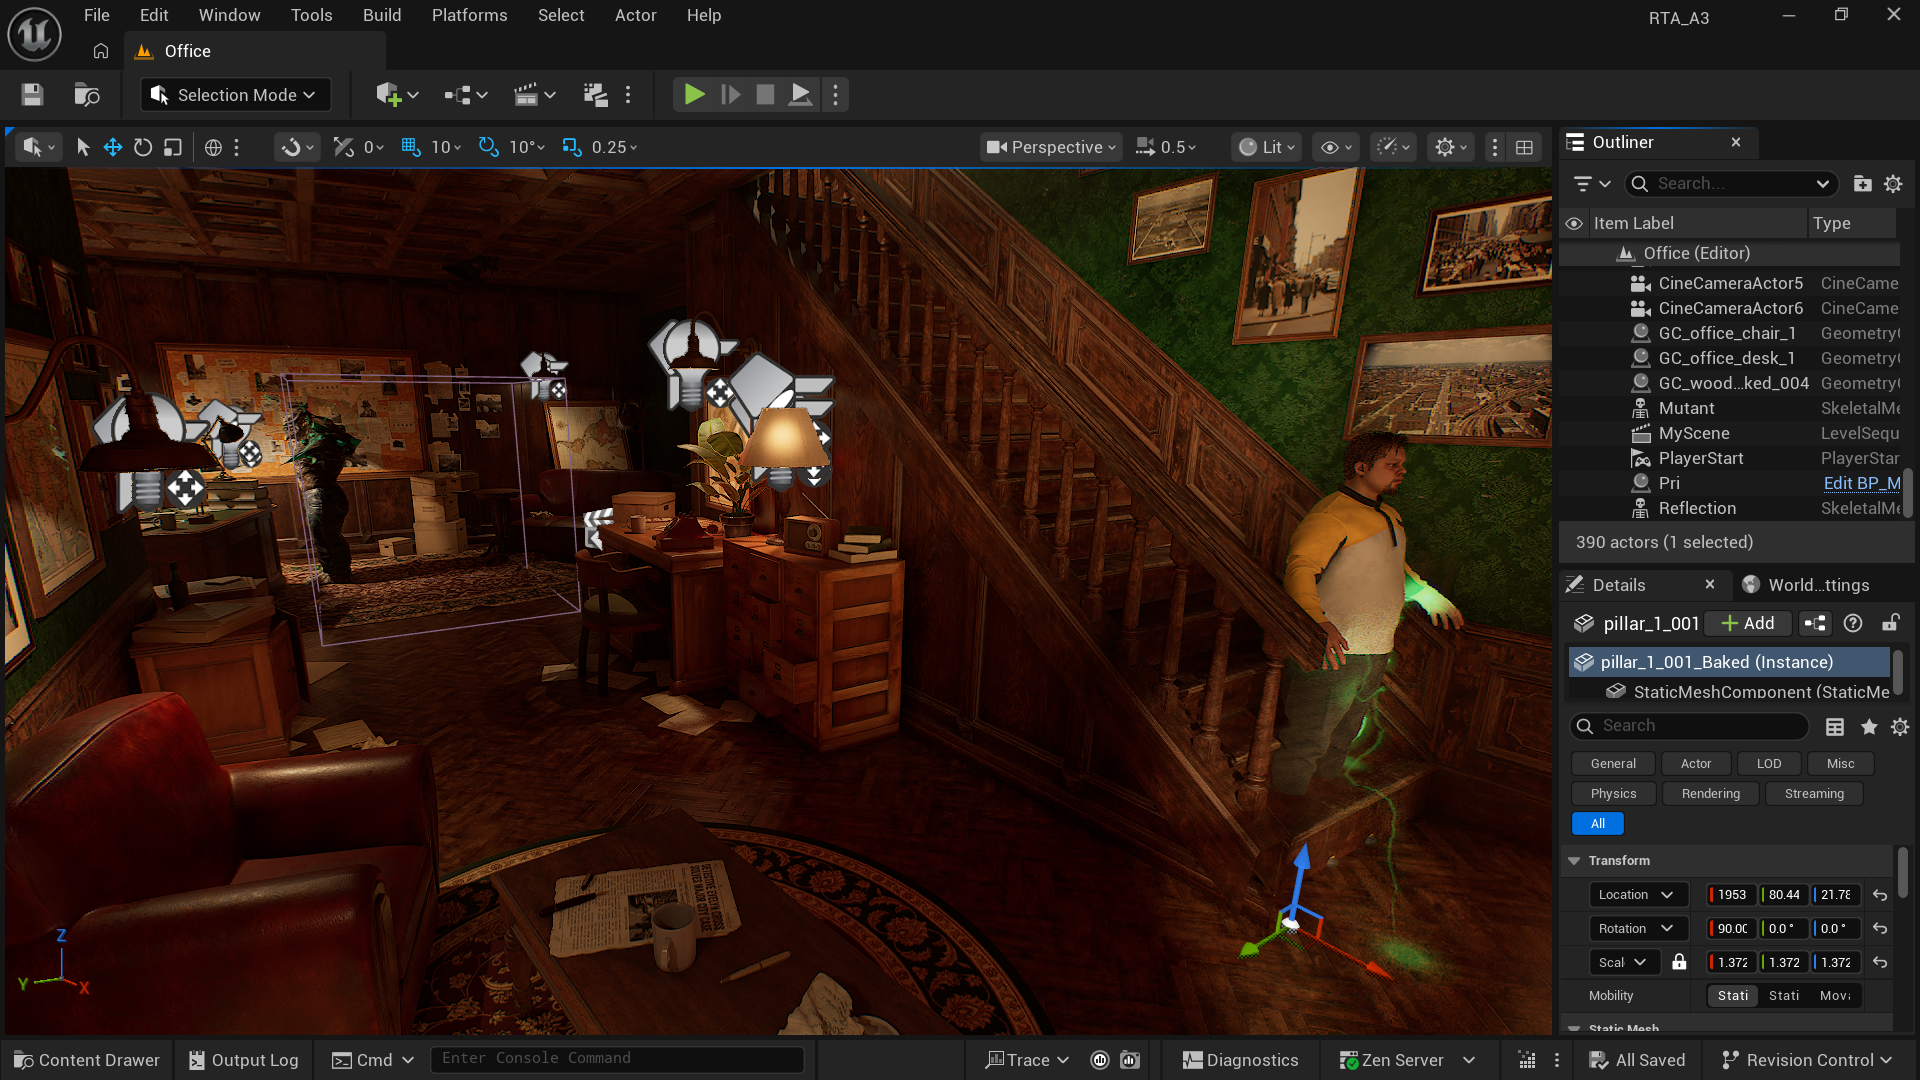
\includegraphics[width=0.9\linewidth]{images/Main Scene.png}
  \caption{Final office scene composition in Unreal Engine 5, showing the detective's home office as the main storytelling and simulation space for the sequence.}
\end{figure}

The story setting is as follows. A detective stands up from the foot of the staircase of his home office after pondering over a mysterious chain of murders that are almost fantastical in nature. He slowly makes his way down the corridor, his mind still clouded with possibilities and theories. As he walks distracted, he catches a flicker of green from the corner of his eye, surrounding an unclear creature reflected in the glass on the door to his garage. Before he can even register it fully, he hears a terrifying roar, causing him to turn around in shock and immense fear, scanning his surroundings and the origin of the sound, yet nothing seems to appear but another flicker of green. Fearful, he turns to face his investigation board to try and make sense of the strange occurrences, when he is suddenly overcome with dizziness. He starts feeling intensely hot, and a strange pain echoes all over his body, while an unnatural smoke begins to emit from him as though heat is escaping through the skin itself. Something is clearly wrong, but before he can overcome the dizziness, a sharp pain washes over his head. He holds his head, shaking violently to let off the screams inside his mind and the immense pain, his body beginning to emit a reddish glow which slowly transitions into the same eerie green as the earlier apparition. Fighting a downward battle against the pain, the man thrashes around, when he is suddenly struck by green lightning from the same hallway where he saw the mysterious figure, causing him to fly backwards and land on his back, stumbling over a pile of boxes. He lies in immense pain, the lightning slowly crawling all over his body, or rather, seeming to emerge from him. However, the man is helpless as the mysterious power takes over, lifting him off the ground, his limbs falling limp in surrender, and then beginning to expand in grotesque ways: his chest and upper body muscles swelling rapidly, his arms and hands becoming heavier and taking on inhuman shapes, and his head inflating unnaturally. The lightning and glow overtake him completely, until an explosion bursts outward from the first impact point on his chest. Amidst the smoke emerges the very monster he had been chasing, the same reflection that had eluded him earlier, now fully materialised, bellowing a grotesque roar as green energy settles around him and a magical glow emits from his body. The mutant leaps forward and lands onto the office desk, shattering it into pieces with barely any effort, while the magical energy surrounding him keeps nearby debris in continuous chaos. He moves forward unfettered and violently uses his now deformed sword-shaped arm to slice apart the cabinet of cases, then punches into the bookshelf with his enlarged hand. This violent visage leaves the room in a chaotic mess, yet just as suddenly as he appeared, the mutant seems to lose his rage, standing stunned for a second before falling flat into the center of the same mess he created. As if the transformation itself is rejecting him, he is overcome by exhaustion and bursts apart in the same kind of explosion that brought him forth, leaving behind only the remains of flesh and ruin, adding yet another unexpected victim to the pile.

\section{Principles of Animation}

My implementation for this scene used a wide range of techniques to achieve the final result. Since the scene is performance-driven, I will first discuss the two main characters and the environment, before listing the key instances in the sequence that correspond to the required principles of animation. One of the biggest goals of the project was to make the story feel authored as a complete sequence rather than a disconnected collection of technical demonstrations, so most of the principles are embedded into the scene progression itself.

\subsection{The Detective}

The main character is a MetaHuman made in my own liking during my Extended Reality lab. Since I was planning on using him in the final RTA assignment anyways, I decided to take this opportunity to learn a few techniques with it in the current project. He comes equipped with a functional body and facial rig, as well as custom free clothing obtained directly from Epic Games \cite{epic_metahuman_docs}.

\begin{figure}[htbp]
  \centering
  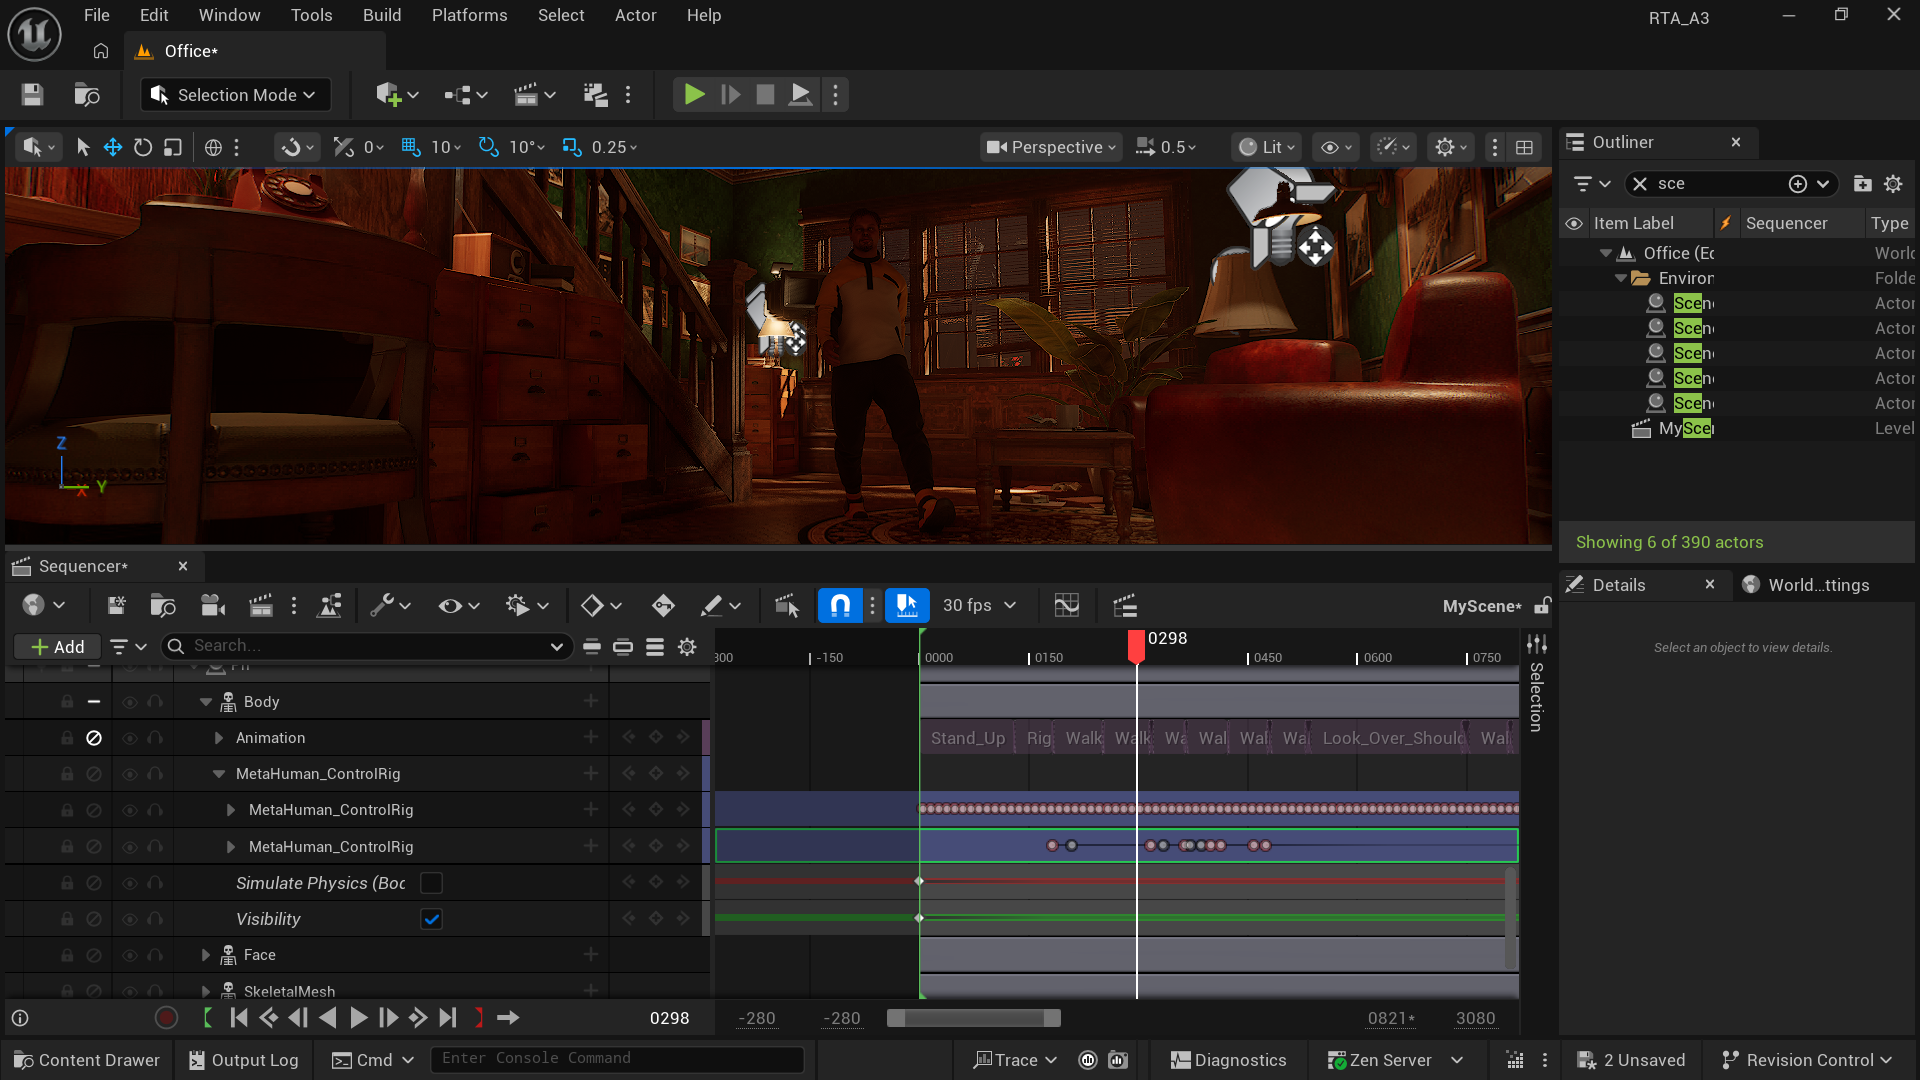
\includegraphics[width=0.7\linewidth]{images/Meta.png}
  \caption{The detective MetaHuman assembled in Sequencer, with retargeted body animation and MetaHuman Control Rig tracks used to refine performance and pose continuity.}
\end{figure}

The approach for animating him used a layered workflow rather than a single technique. After receiving permission to use base skeletal animations for simple actions from Mixamo, I selected a set of clips suited to the story, such as standing, walking, reacting, stumbling, falling, and writhing in pain \cite{mixamo_motion,metahuman_animation_list}. Each animation was retargeted to suit the MetaHuman skeletal structure \cite{epic_ik_rig_retargeting}, after which I assembled the overall sequence directly in Sequencer.

The key challenge here was that base clips are only a starting point. When unrelated source animations are placed back-to-back, the seams between them become visible through foot sliding, body jitter, abrupt rotation shifts, and inconsistent posing. To solve this, I matched successive animations using Sequencer's clip matching tools, aligning clips by selecting appropriate bones from the previous section and choosing whether to match translation and rotation depending on the movement context. In walking transitions, foot and root alignment were especially important to preserve continuity and reduce snapping between clips. This gave me a workable baseline.

Once the rough assembly was in place, I baked the transforms and rotations of the sequence so that the overall movement could be edited as a more coherent performance. I then baked the full character motion into the MetaHuman Control Rig. This was one of the most important steps in the project, because it transformed the detective's animation from a chain of retargeted source clips into something I could shape shot-by-shot. Through the Control Rig, I was able to do a second pass using a combination of forward and inverse kinematics to correct awkward poses, reduce visible jitter introduced by blending, and push certain scenes beyond what the source animations originally offered \cite{youtube_control_rig,epic_control_rig_animating}. This was especially useful in scenes involving walking, shock, dizziness, violent headache, and the transformation itself, where I needed more precise control over limbs, torso, body offset, and balance than a standard retargeted clip could provide.

The Control Rig pass also helped me manipulate the detective's body in more exaggerated and dramatic ways during the transformation. Selected controls were repositioned, rotated, and in some cases scaled to distort the body gradually as the sequence intensified. This made the transformation feel like an authored physical event rather than simply a visual effect layered on top of a normal animation. His skeleton also later served as a useful target source for Niagara systems, allowing smoke, glow, and lightning to appear attached to the body in meaningful places rather than floating randomly around him.

\subsection{The Mutant}

The mutant is both the deuteragonist and the antagonist of the scene. Taken from a free character asset from Mixamo together with its own set of base animations, it functions first as the source of paranoia and later as the fully realised aftermath of the detective's transformation \cite{mixamo_character,mixamo_motion,mutant_animation_list}. Like the detective, the mutant came with its own skeletal structure, so I followed a similar process of building a full sequence from multiple animations, blending and matching them in Sequencer, and then adjusting transforms and timings to shape the performance.

\begin{figure}[htbp]
  \centering
  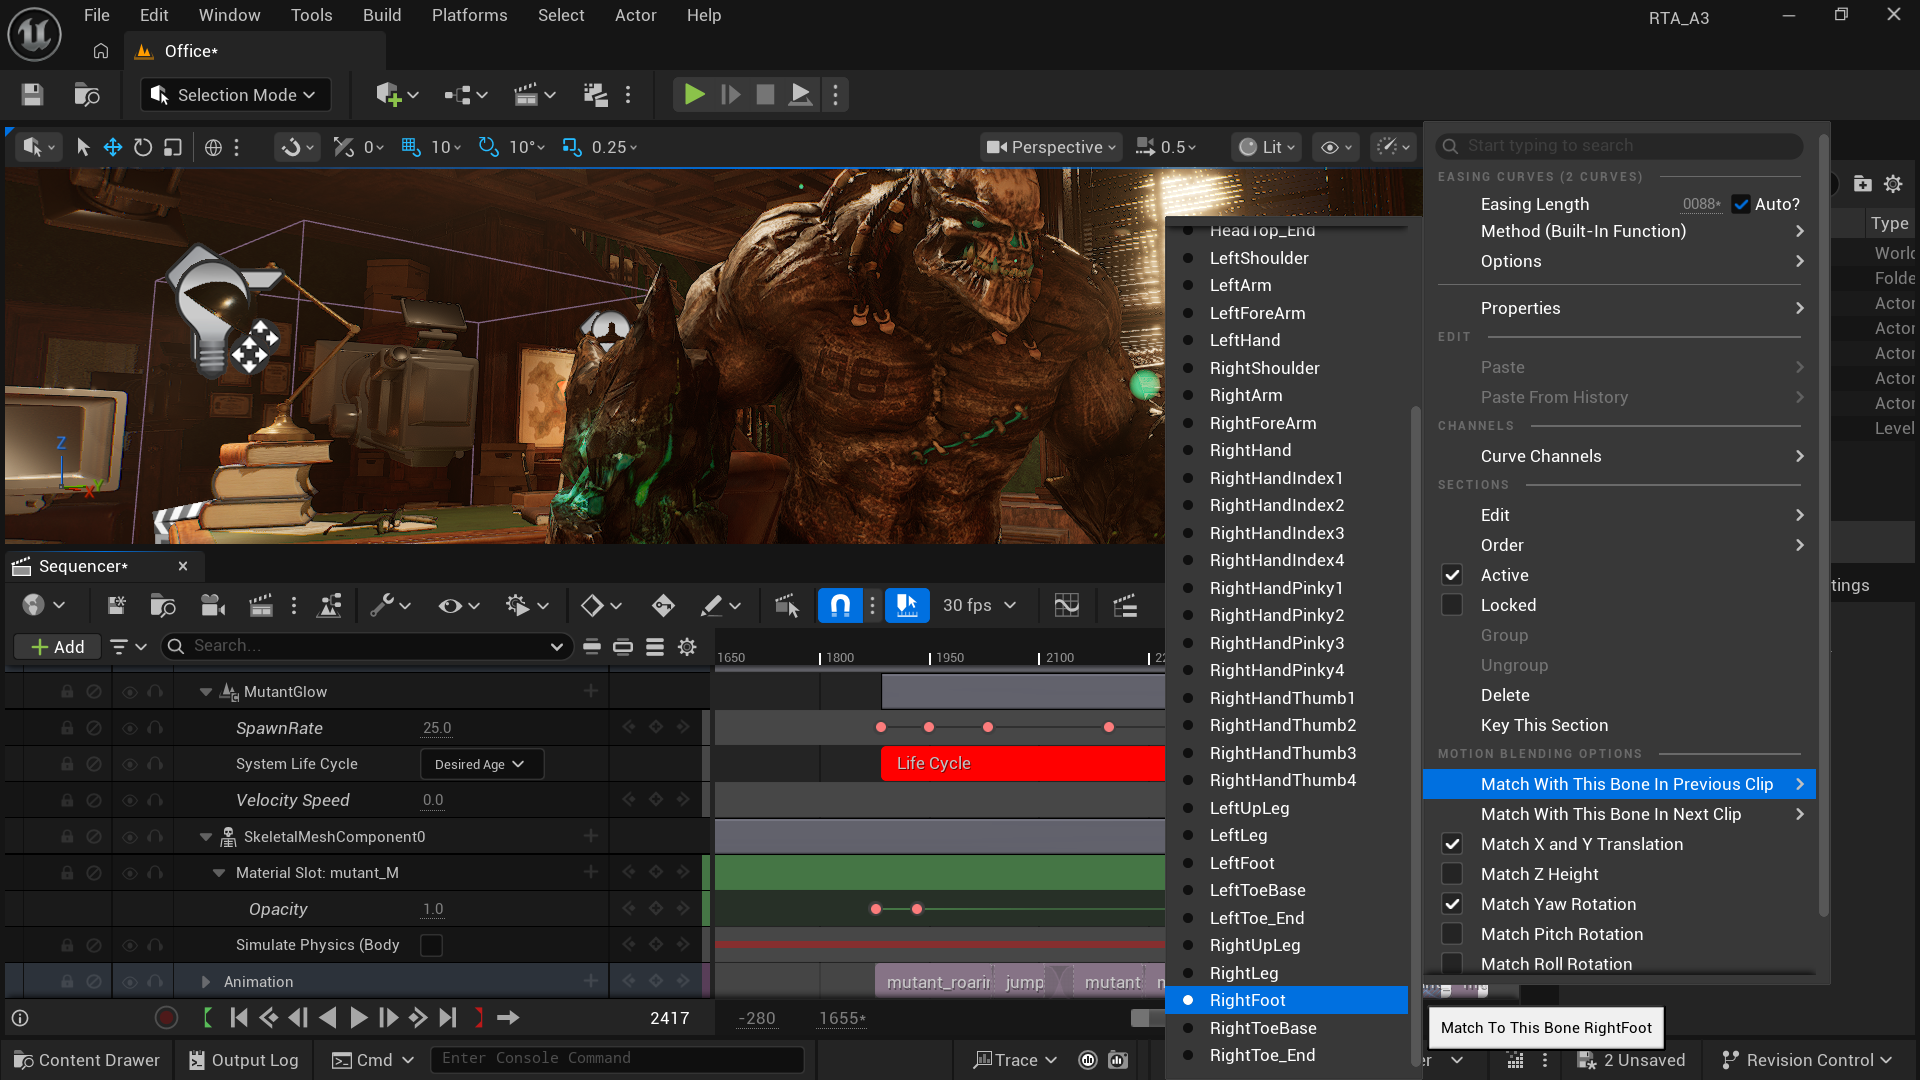
\includegraphics[width=0.7\linewidth]{images/Mutant 2.png}
  \caption{The mutant performance inside Sequencer, showing layered animation, Niagara glow control, material opacity animation, and bone-based clip matching during aggressive action beats.}
\end{figure}

However, the mutant's motion had a very different purpose. While the detective required a more human and readable acting performance, the mutant needed to feel heavy, unstable, powerful, and unnatural. This meant pushing anticipation and follow-through more aggressively, lengthening attack windups, and exaggerating body mechanics during roars, leaps, slashes, and heavy impacts. I also adjusted body motion in ways that prioritised force and menace over realism, so that even when relying on sourced clips, the mutant felt like a chaotic creature.

In addition to the main mutant that appears after the transformation, a secondary instance of the mutant was placed behind the gated hallway glass of the house. This was used for the earlier hallucination scene. Its appearance and disappearance were controlled by modifying the material with a dither temporal fade setup, allowing me to animate opacity in Sequencer. This became a very useful storytelling device, as rather than abruptly spawning or hiding the creature, I could make it appear into view as a reflection-like hallucination, then later reuse the same logic to fake the mutant's entrance and disappearance during the transformation sequence itself.

The mutant's skeletal mesh component was also enhanced with collision and physical interaction so that it could interact with nearby props during destruction segments, combining the mutant's aggressive motion with rigid body props and fractured objects, and allowing the environment to react in a way that supported his weight and violence.

\subsection{The Environment}

For the sake of simplicity and time constraints, the environment was built using free assets from the Fab marketplace \cite{fab_detective_office}. These were arranged and lit to create a compact but visually dense home office. Since my device has limited performance, I reduced texture quality where needed and tuned post-processing, point lights, and area lights to create the atmosphere without making the scene unreadable. Boxes, books, papers, desks, cabinets, shelves, and clutter were positioned in a way that made them useful both for believable detective space and for collision-driven reactions.

\subsection{Instances of the Principles of Animation}

There are a wide number of scenes that instantiated the four required principles.

\begin{figure}[htbp]
  \centering
  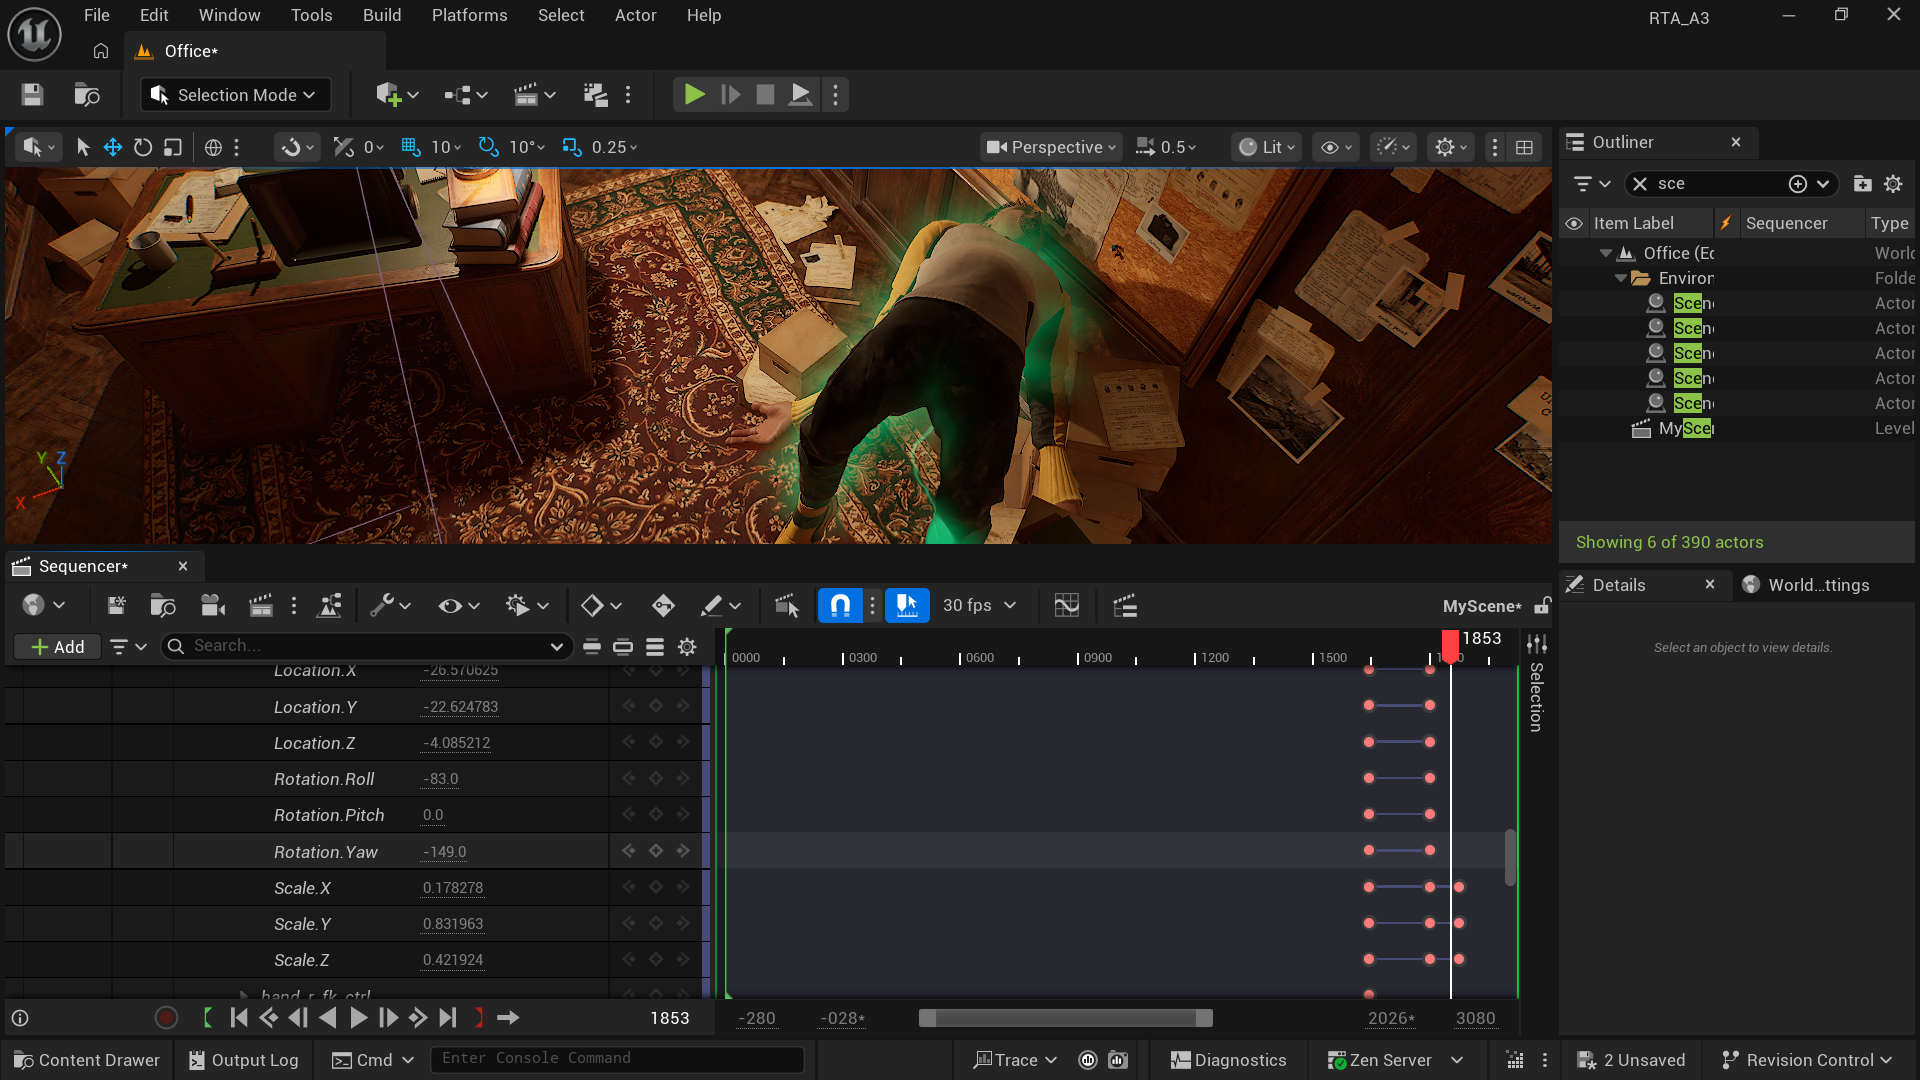
\includegraphics[width=0.82\linewidth]{images/Squash and Strethc.png}
  \caption{Control Rig deformation and body scaling during the transformation sequence, used to communicate stretch, compression, and unnatural physical change.}
\end{figure}

\subsubsection{Squash and Stretch}

\begin{itemize}[leftmargin=*]
  \item Body compression when the detective lands after the lightning strike.
  \item Slight stretch during the first lightning impact and backward launch.
  \item Expansion of spine, clavicle, arms, hands, neck, and head at different degrees during the transformation sequence.
  \item Body reshaping through Control Rig adjustments to make animations more physically expressive.
  \item Very subtle compression and stretching of the mutant during selected heavy actions.
\end{itemize}

\begin{figure}[htbp]
  \centering
  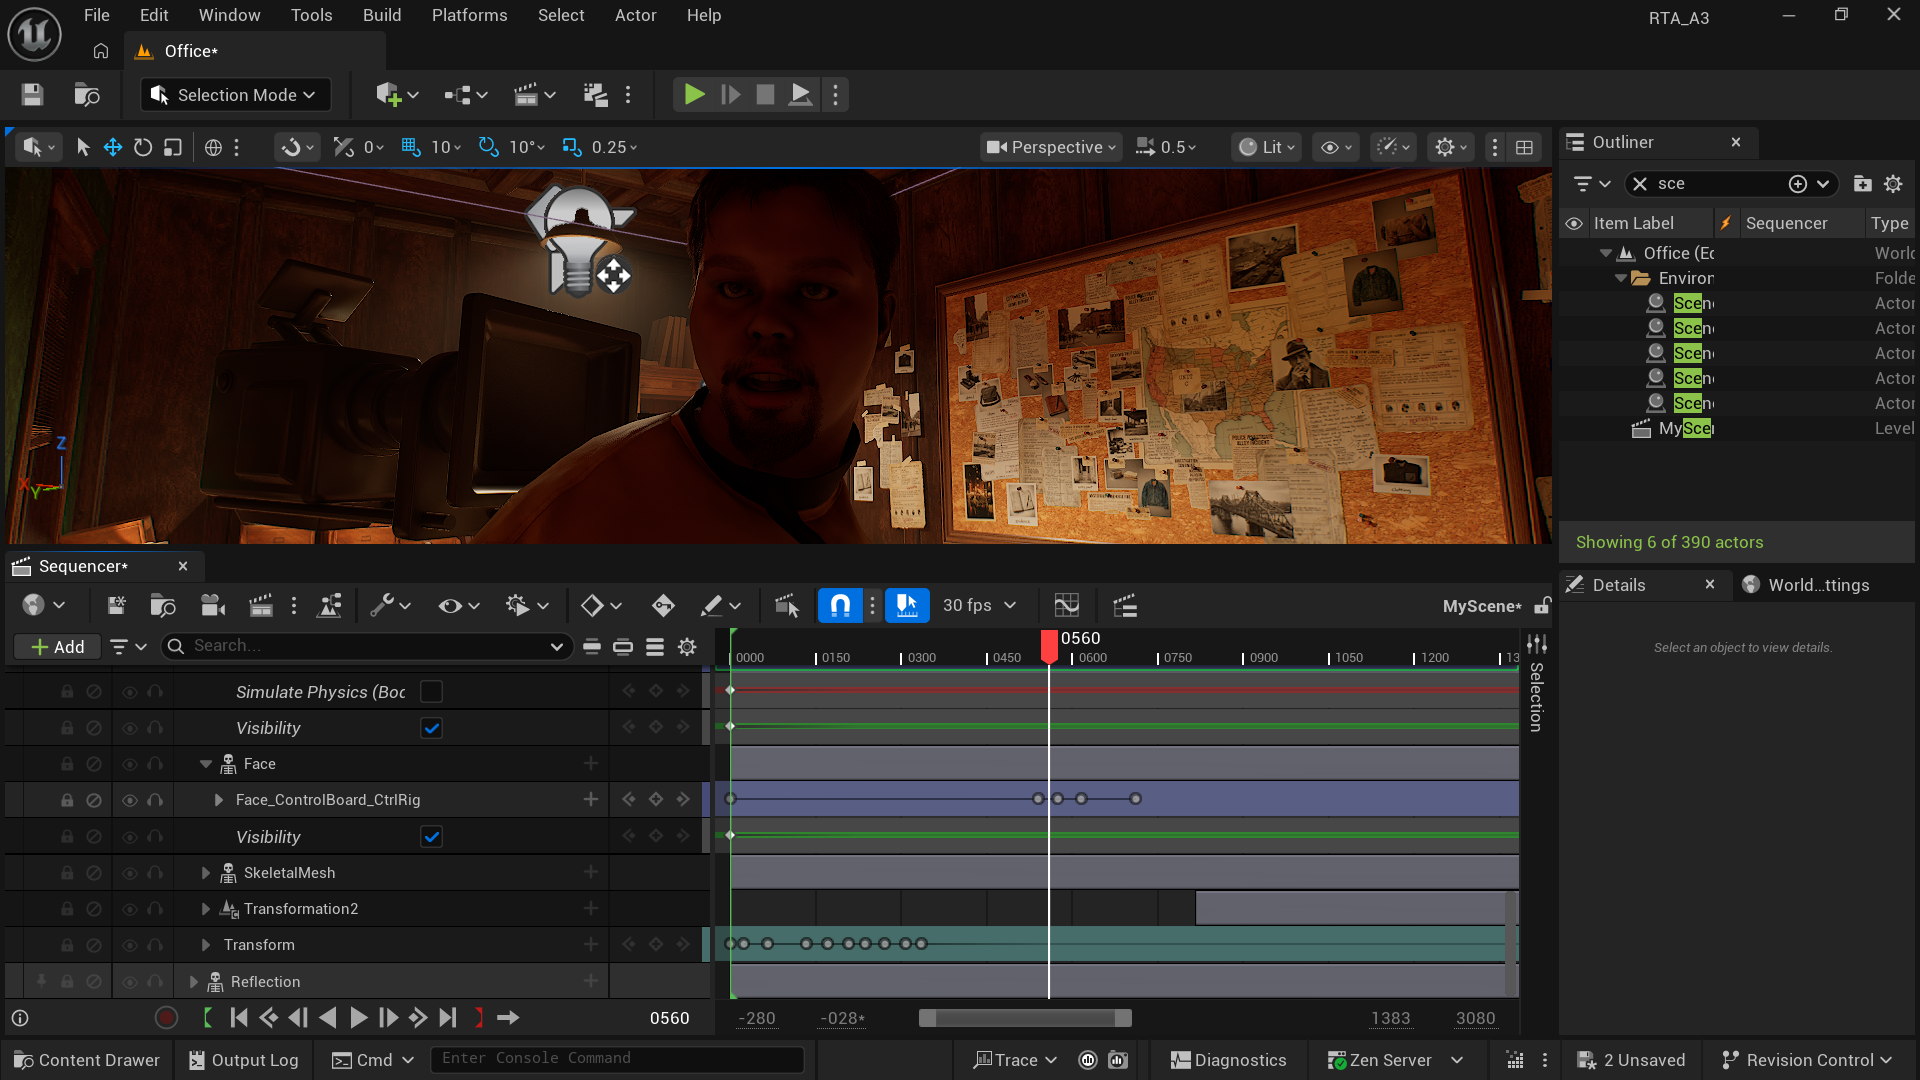
\includegraphics[width=0.82\linewidth]{images/Anticipation.png}
  \caption{A held pre-action pose in Sequencer, where timing and body posture are used to build anticipation before the detective's next movement beat.}
\end{figure}

\subsubsection{Anticipation}

\begin{itemize}[leftmargin=*]
  \item Main character pauses after standing up and before starting to walk down the corridor.
  \item He hesitates after seeing the mutant's reflection and after hearing the roar.
  \item There is a delay in his shock reaction, with the body and face preparing before the full turn and recoil.
  \item The transformation is preceded by a dizziness buildup.
  \item Holding his head and staggering act as anticipatory action.
  \item Body tenses and recoils before and after being flung backward.
  \item Mutant uses preparatory windup poses to make the attacks feel stronger.
\end{itemize}

\begin{figure}[htbp]
  \centering
  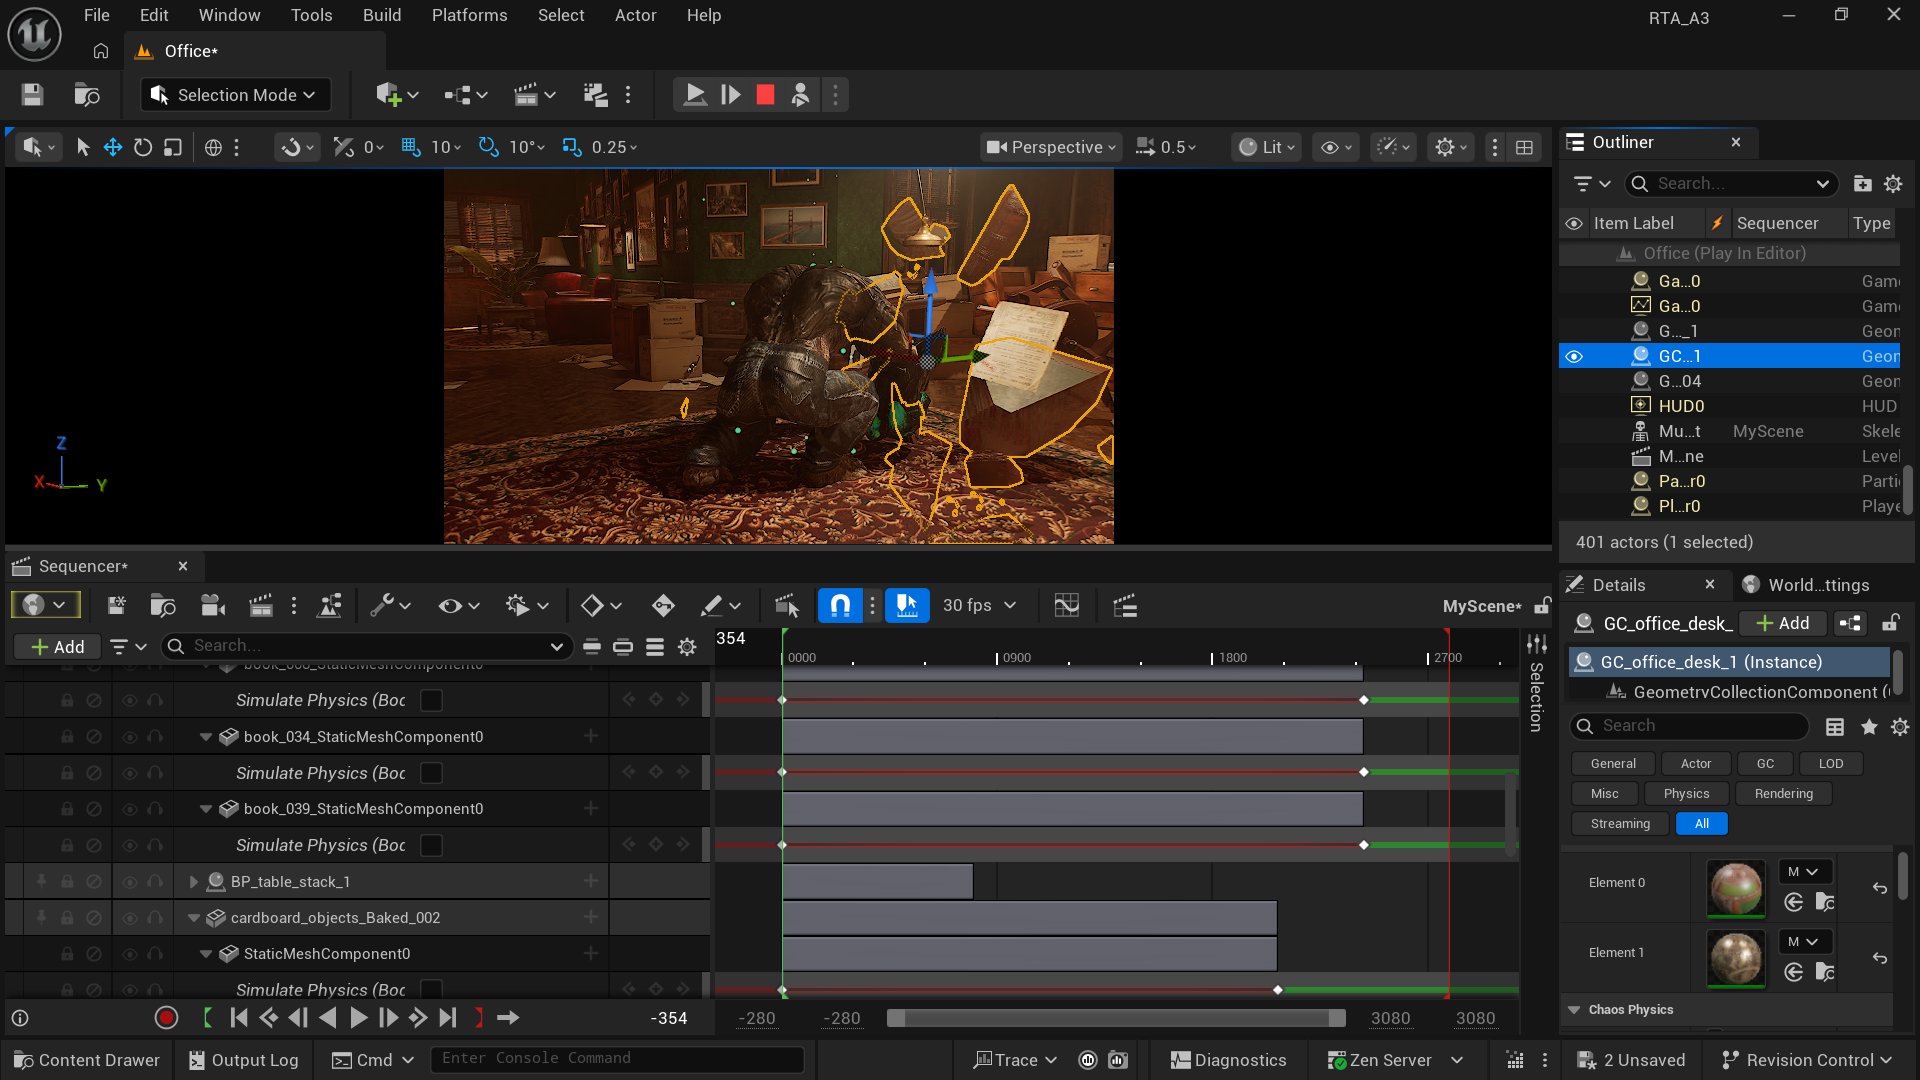
\includegraphics[width=0.82\linewidth]{images/Follow Through.png}
  \caption{Follow-through after impact, with the detective's body continuing to settle and react after the main action rather than stopping immediately.}
\end{figure}

\subsubsection{Follow Through}

\begin{itemize}[leftmargin=*]
  \item Body ragging during dizziness and after sudden reactions.
  \item Arms, posture, and facial features continue to adjust after the shock moment instead of freezing immediately.
  \item After the detective is thrown back, the body continues to react and struggle on the ground.
  \item Boxes falling after table contact due to collision.
  \item Transformation sequence continues to evolve through particle buildup and body motion.
  \item Props scatter on hit and continue sliding, tumbling, or falling.
  \item Destruction fragments and debris continue to move after the mutant's attack.
\end{itemize}

\subsubsection{Exaggeration}

\begin{itemize}[leftmargin=*]
  \item Shock reaction uses widened eyes, open mouth, neck tension, and strong torso rotation.
  \item Arm and head movements are pushed further to simulate fear and pain.
  \item Violent head pain and body convulsions are deliberately heightened.
  \item The lightning strike launches the body backwards in an intense way.
  \item Mutant roar pose is theatrical.
  \item The leap attack, desk break, cabinet slash, and bookshelf punch all push force beyond realism to communicate monstrous power.
\end{itemize}

\begin{figure}[htbp]
  \centering
  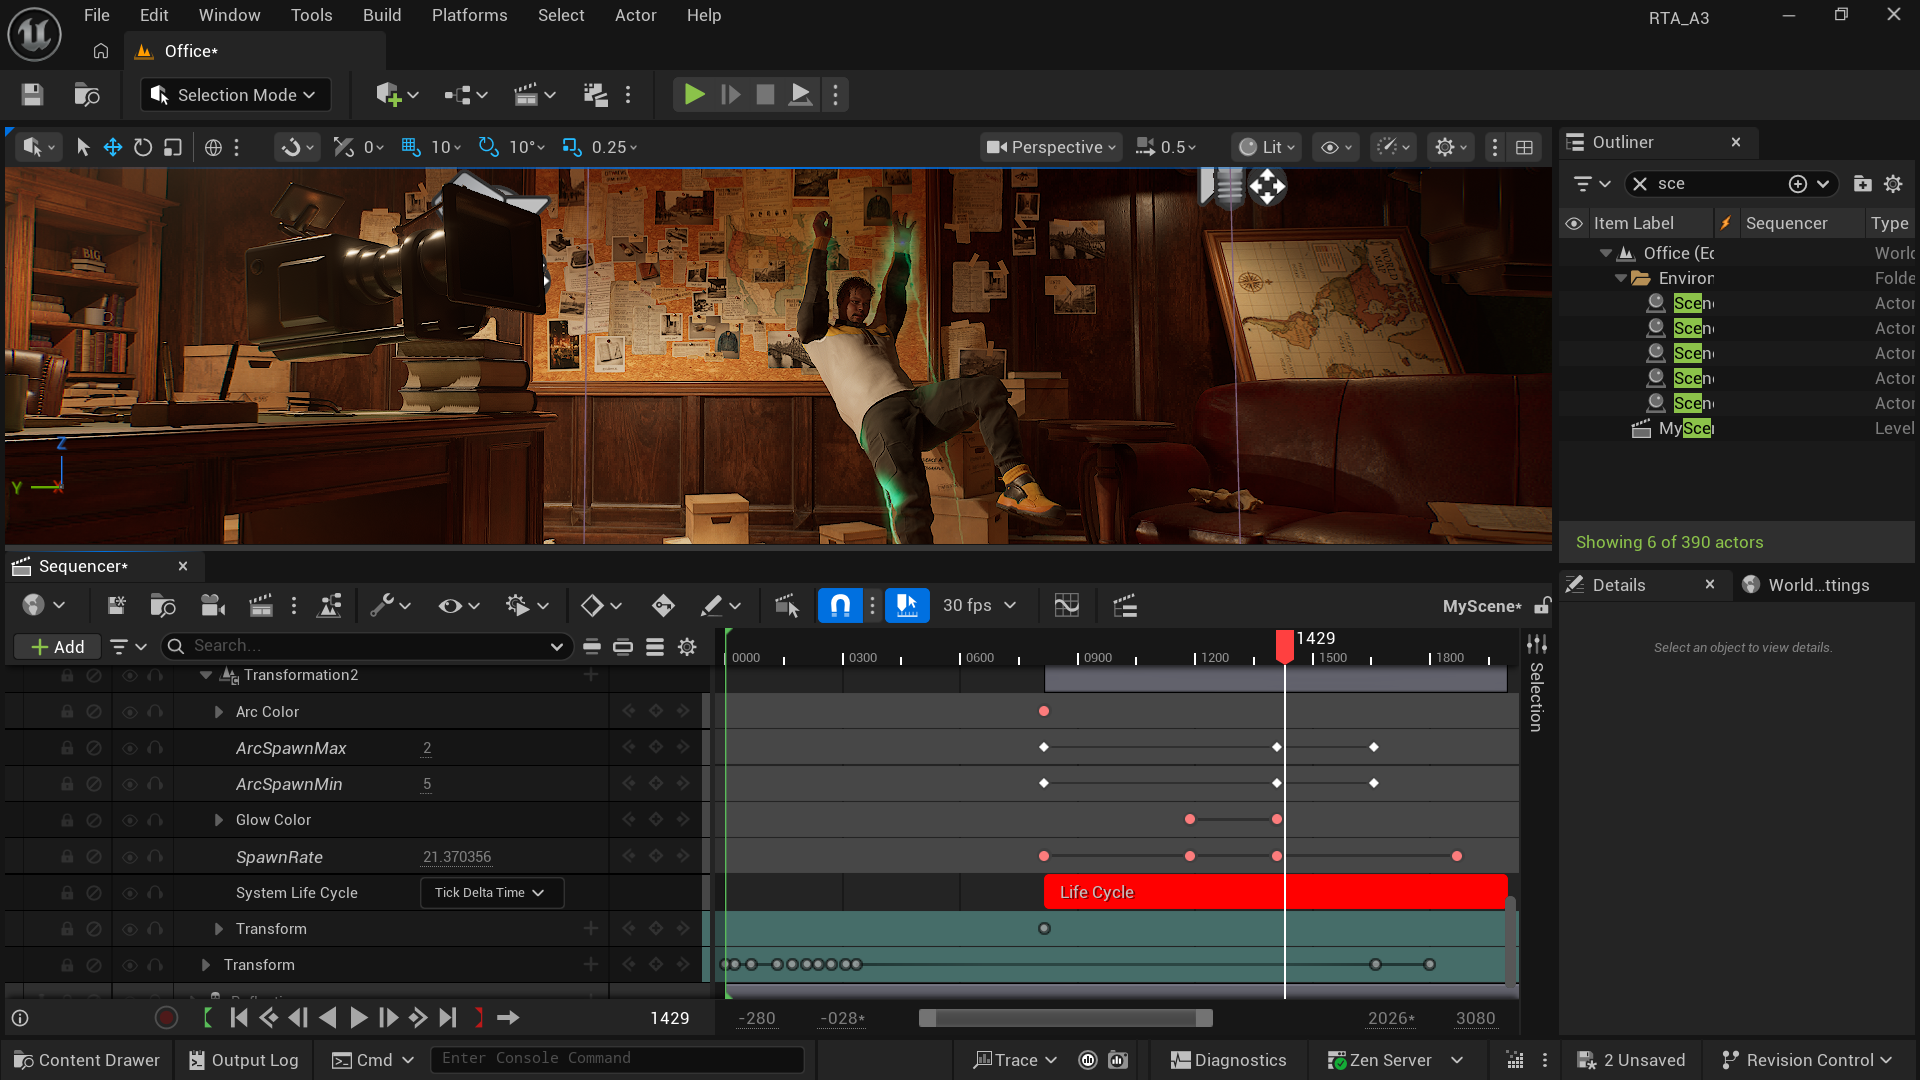
\includegraphics[width=0.82\linewidth]{images/Exaggeration.png}
  \caption{Close-up exaggerated acting in the detective's shock reaction, using facial expression, head movement, and upper-body pose to heighten fear and dramatic clarity.}
\end{figure}

\section{Physically-Based Animation}

I ended up implementing more than just two physically-based animation techniques to enhance my overall scene. The two most prominent ones are discussed first, while a few smaller overlaps are mentioned where relevant.


\begin{figure}[htbp]
  \centering
  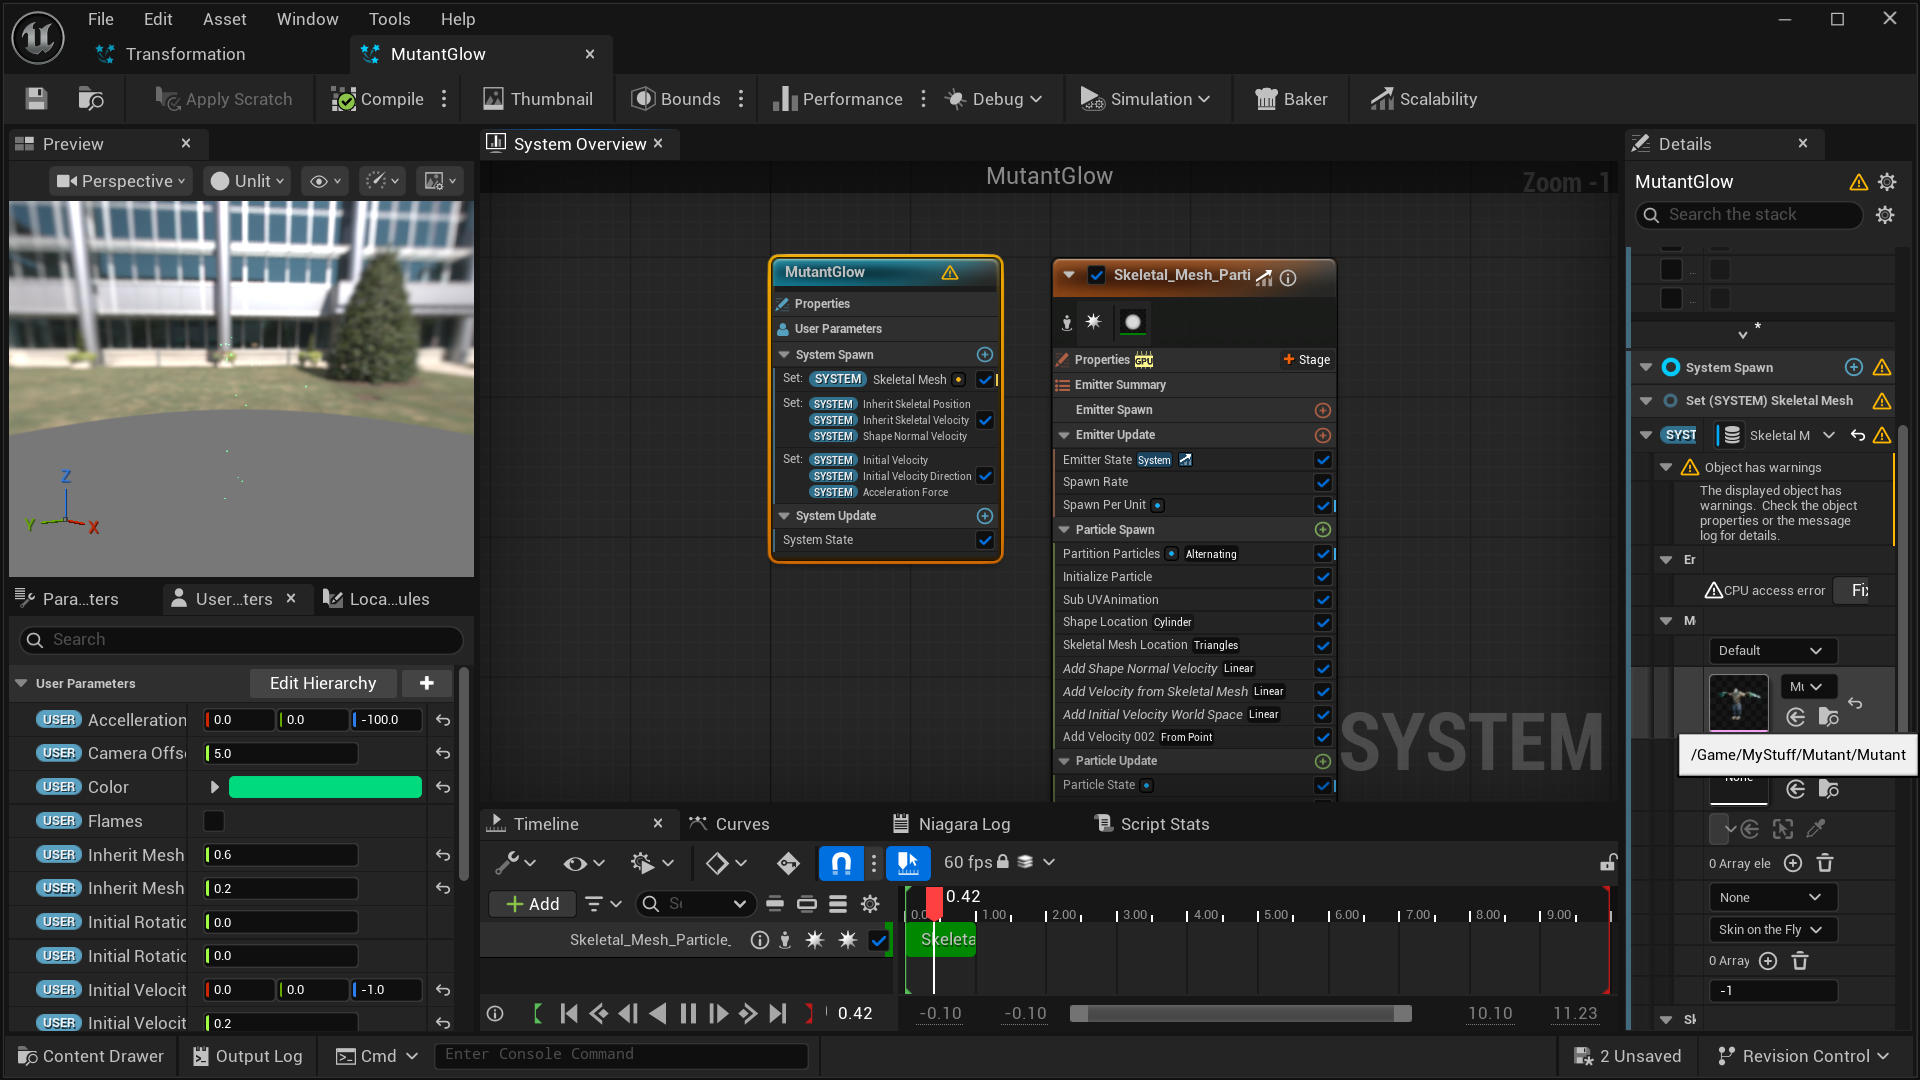
\includegraphics[width=0.8\linewidth]{images/Glow.png}
  \caption{The MutantGlow Niagara system, configured to emit particles from the mutant skeletal mesh so the supernatural aura follows the animated body.}
\end{figure}

\subsection{Particle Systems}

The most prominent technique used to enhance my scene was a series of three Niagara systems.

The simplest one was a glowing effect generated over the mutant's body, featuring glowing green orbs emitting from the mesh. This system was built by studying examples from Unreal's free Niagara example content and then adapting that logic into my own skeletal-mesh-driven version \cite{fab_niagara_examples,epic_niagara_docs}. The particles inherit the general movement of the mesh, which makes the system easy to retarget and use across animations. I exposed parameters such as spawn rate and particle velocity to control in Sequencer, making the effect subtle during moments of suspense and much more aggressive during the mutant's destructive actions, giving the creature an unstable magical aura.

The second and most important Niagara setup was the transformation effect on the detective, which was implemented as a layered, three-part system. The first component is smoke emission attached to the skeleton of the MetaHuman, used to create a steam-like effect, as if heat were escaping directly from the body. The second component is the body glow sequence, adapted from an example that originally behaved more like an instantaneous burst, and I reworked it into a more progressive and spotty pattern that emerges over time. I exposed colour and spawn behaviour so the effect could begin with a blood-red glow and gradually turn green as the transformation advances. The spawn rate was also animated to increase in intensity, allowing the visual energy to grow alongside the character's physical distress. The third component is the lightning from a tesla coil example. This was targeted from an exposed root transform and configured so that arcs could reach towards different bone areas, sometimes between bones, with parameterised minimum and maximum ranges controlling the number and aggressiveness of the arcs. I also exposed colour and spawn-rate related settings so that the lightning could escalate from occasional strikes into a chaotic network all over the detective's body \cite{fab_niagara_examples,epic_niagara_docs}.



\begin{figure}[htbp]
  \centering
  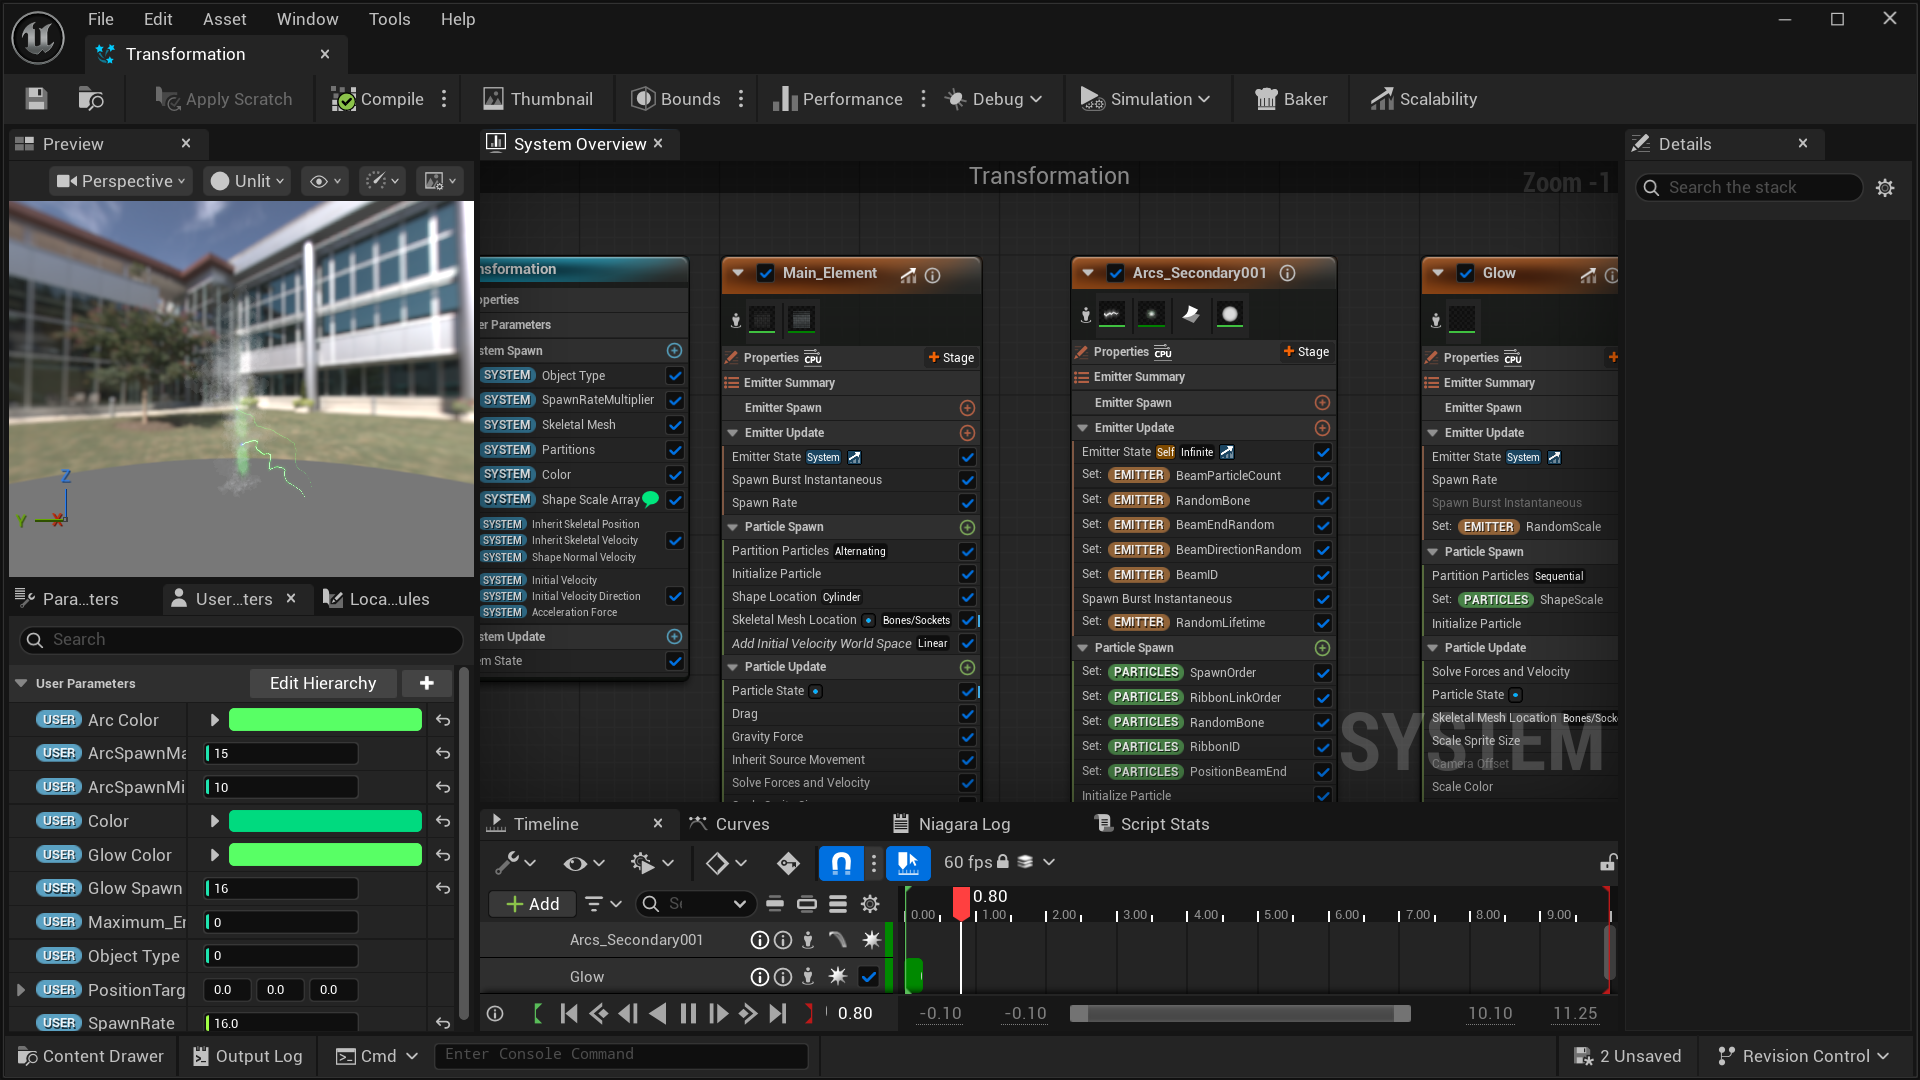
\includegraphics[width=0.82\linewidth]{images/Transformation.png}
  \caption{The main transformation Niagara setup, combining smoke, glow, and electrical arc emitters with exposed user parameters for timing and intensity control.}
\end{figure}

\subsubsection{Smoke and Fire}

The third particle system more appropriately falls under this category, which was a more last-minute addition to represent the explosion used during transformation and the mutant's death. Once again, originating from an example, I followed the official documentation for fire and explosion styling and reworked it into a multi-component spherical explosion that originates from a fixed transform point rather than a cone-based directional burst \cite{epic_niagara_docs,youtube_fire_glow}. It gave me control over smoke, dust, debris, and fire to create a blend to conceal the transition for the two characters' visibility. Unlike the previous two systems, most of this effect's tuning was done directly inside Niagara rather than in Sequencer.

\subsubsection*{Review}

The main limitation across all systems was balancing the effect with readability. If the systems became too dense, the body performance was obscured; if they were too subtle, the transformation lost impact. This required a significant amount of iteration. Even so, this was one of the most successful parts of the project because it combined technical control with strong visual payoff. I was especially grateful for access to strong bases from Epic Games for this, as the example packs allowed for a high degree of customization, with a proper demo scene to see what each of the example systems was supposed to look like to match expectations \cite{fab_niagara_examples}. Because of parameterisation I could choreograph effects in the same timeline as the character performance.

\subsection{Rigidbody Physics}

\begin{figure}[htbp]
  \centering
  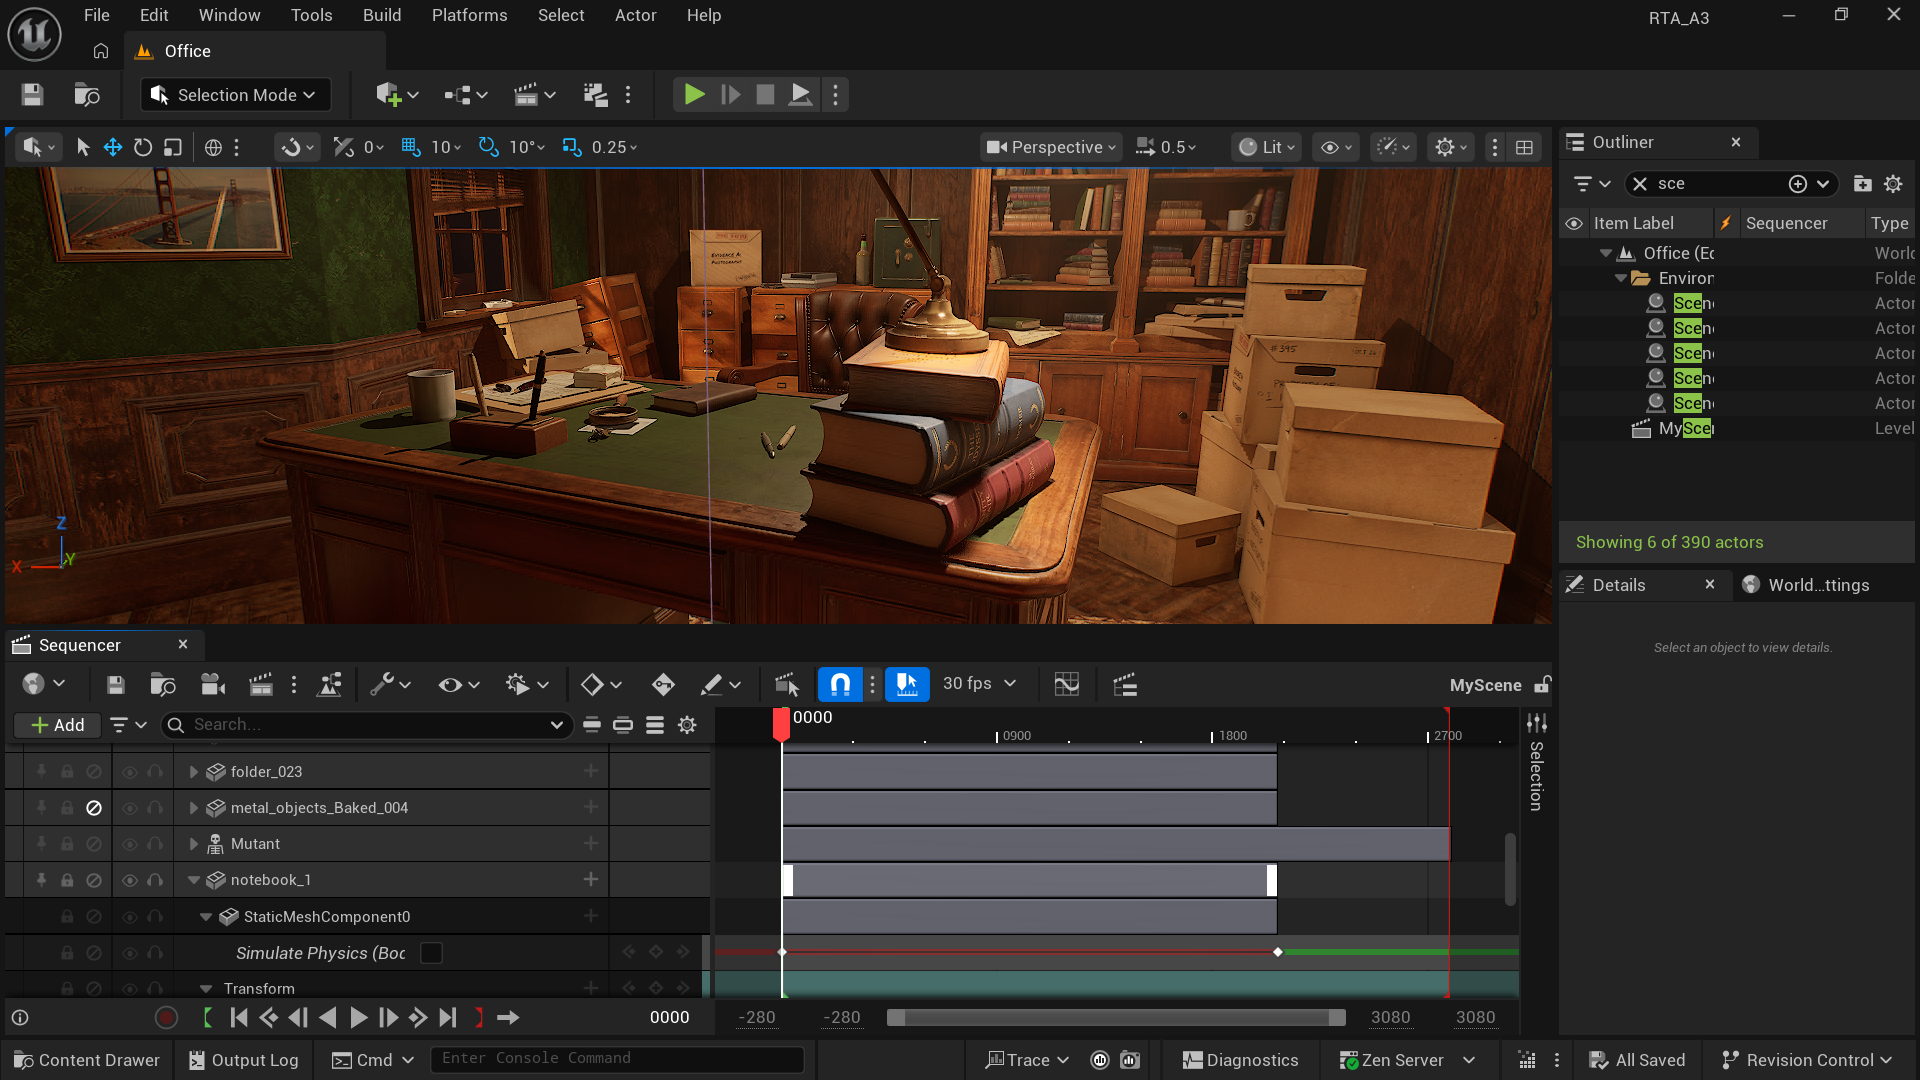
\includegraphics[width=0.82\linewidth]{images/Rigidbody.png}
  \caption{Rigid body interaction staged in Sequencer, with selectively activated simulation used to drive prop motion and environmental response during impact moments.}
\end{figure}

The second main physically-based animation technique was rigid body physics, though in practice this also overlapped with character-driven interaction, force-based motion, and destruction. By default, collision and rigid body interaction were enabled where useful in the characters' skeletal mesh components to help support meaningful interactions with the environment. However, the main use of rigid body simulation in the final sequence came from props and set pieces.

Rather than hand-keyframing every environmental reaction, I used physics selectively through Sequencer. Specific keyframed instances activated simulation on props only when needed, for both isolated static meshes or collections of them grouped into actor blueprints. This allowed objects to react to collisions and impacts during the scene while remaining manageable from a cinematic perspective.

At the same time, this system was the least predictable part of the project. Despite various attempts to tune collisions and physics behaviour, some inconsistencies remained. In the final scene, some boxes clip into the body despite having collision enabled, and some smaller meshes such as lamps or books occasionally linger unnaturally in the air instead of reacting exactly as intended. Even though this made the system less stable than purely keyframed animation, it still contributed significantly to the feeling of physical interaction and mess.

\subsubsection{Destruction}

\begin{figure}[htbp]
  \centering
  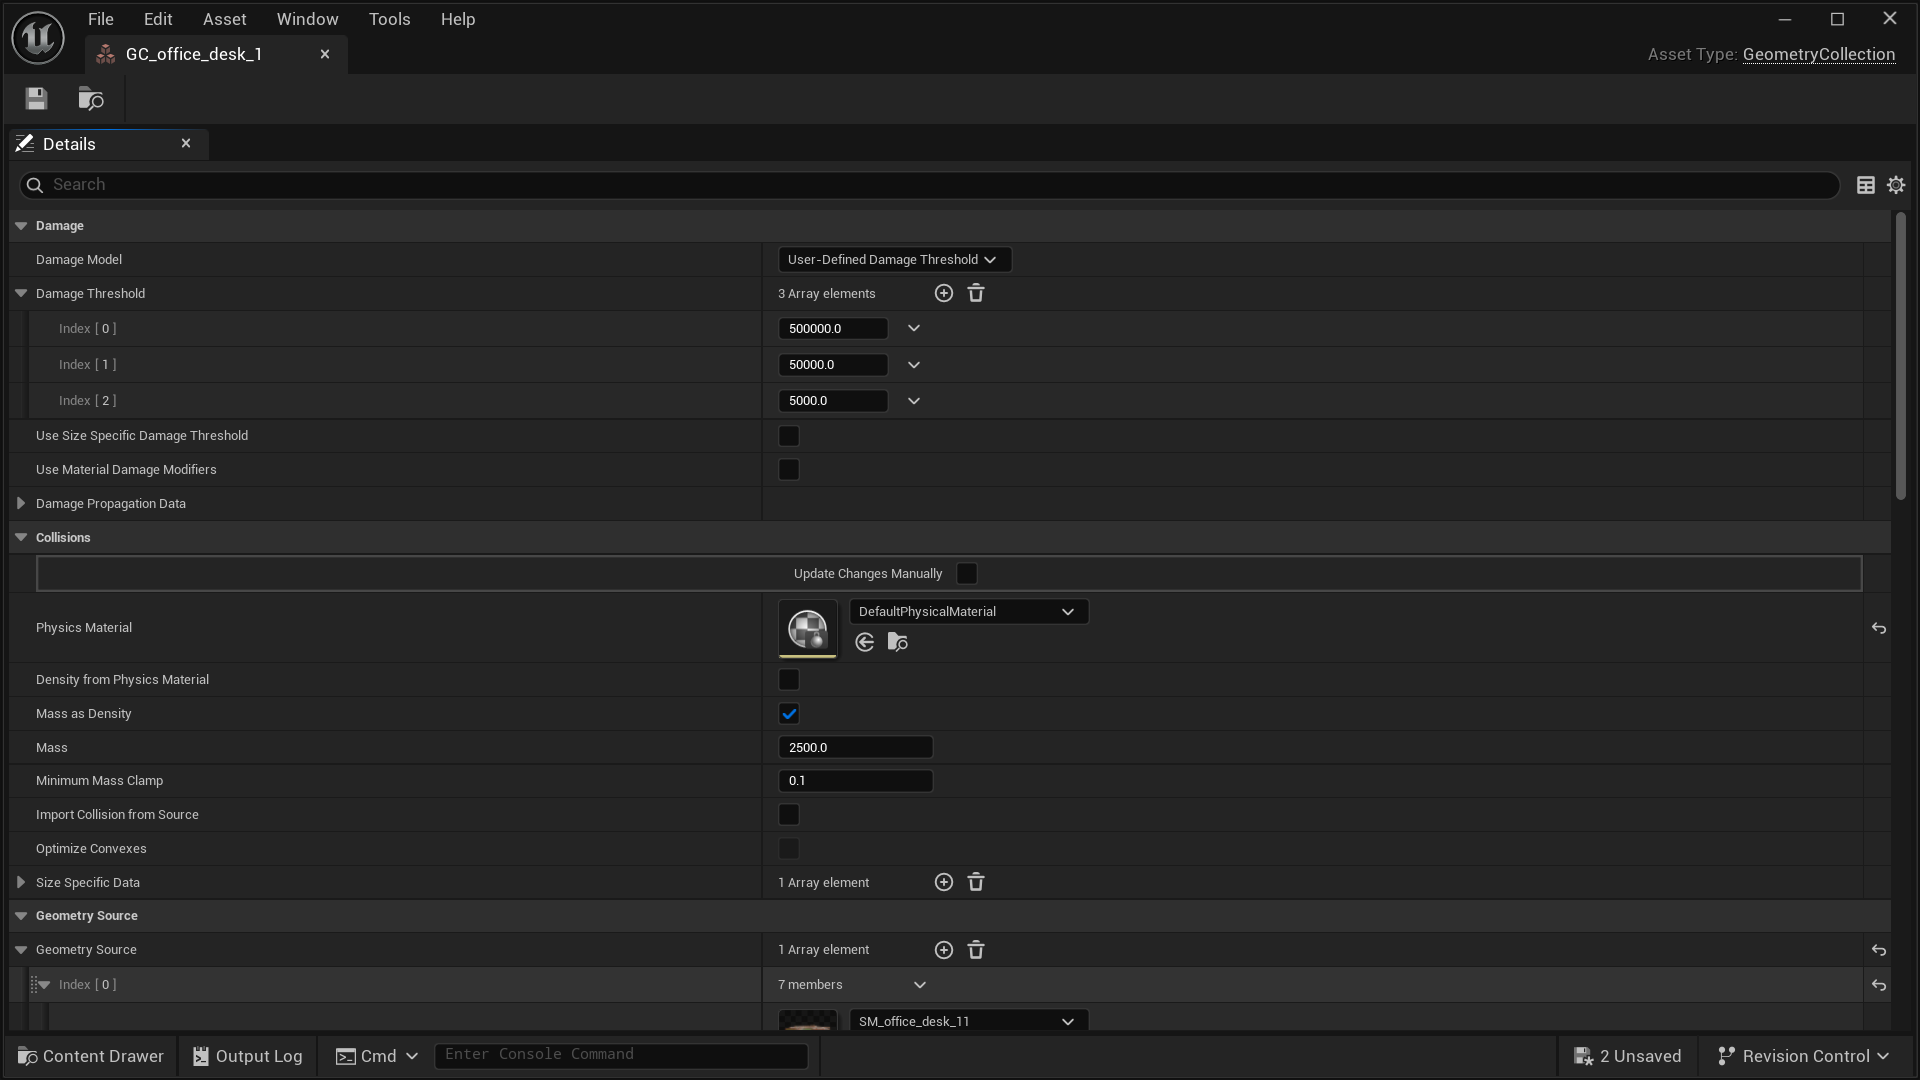
\includegraphics[width=0.82\linewidth]{images/Destruction.png}
  \caption{Chaos destruction and fractured geometry reacting to the mutant's attack, extending the action into the office environment through debris and material breakup.}
\end{figure}

A specific subset of rigidbody physics was Chaos destruction through fracture and Geometry Collections. I created three different Geometry Collections to simulate destruction in major mutant attack moments. These were fractured either using uniform settings with up to two levels of fragmentation where useful \cite{epic_chaos_destruction}. They were keyed at the appropriate moments using Sequencer to keep the scene stable before the impact while still allowing violent destruction once the mutant attacked. I found this more effective than simply throwing around intact static meshes, because it produced fragments, debris, and a stronger visual sense of force. An added advantage of this setup was that some destructible objects also served as bases for other physics-enabled props, allowing secondary items to be flung around as a byproduct of the fracture event.

\subsubsection*{Review}

Rigid body simulation and destruction greatly improved the scene because they extended the mutant's actions into the environment. Without them, the attacks would have relied too heavily on the mutant's own animation and would have lacked a convincing sense of impact. The main challenge was consistency. Unlike hand-authored animation, physics can behave unpredictably, particularly in a cluttered environment with multiple nearby objects and different collision relationships. This was both a strength and a weakness.
\newpage
\section{References}

\nocite{*}
\printbibliography[heading=none]

\end{document}